\cleardoublepage
\chapter{Optimizing Oxygen Input Profiles for Efficient Estimation of Michaelis-Menten Respiration Models}
\label{paper1}
This chapter has been published in Food and Bioprocess Technology.\footnote{\textbf{Strouwen, A.}, Nicolaï, B.M., Goos, P. (2019). Optimizing Oxygen Input Profiles for Efficient Estimation of Michaelis-Menten Respiration Models. Food and Bioprocess Technology, 12 (5), 769-780. }
\\
\\
{\color{red}Source code available upon request.}
\section*{Abstract}
Models based on mass balances and Michaelis-Menten respiration kinetics are increasingly used to determine optimal storage conditions of fresh fruits and vegetables. The model parameters are usually estimated from respiration experiments at different, but fixed, gas conditions according to a response surface design. This is a tedious procedure that requires a gas mixing facility or a series of gas cylinders with appropriate composition. In this chapter, we consider a simpler approach, in which the respiration kinetics of pear fruit are modeled using a single experiment with a time varying $\text{O}_2$ input profile. To optimize the information content produced by the $\text{O}_2$ profile, we apply optimal dynamic experimental design principles and present a modified coordinate-exchange algorithm to achieve this goal. Finally, we demonstrate the added value of our approach by comparing the optimal $\text{O}_2$ input profiles to several intuitive benchmark experiments.
\section{Introduction}
Fresh fruit needs to be stored at appropriate temperature as well as $\text{O}_2$ and $\text{CO}_2$ conditions, after its harvest. The ideal storage conditions depend on the species, cultivar, ripeness stage and many other factors, and must be experimentally determined. Traditionally, this is achieved by independently storing fruit at many different combinations of temperature as well as $\text{O}_2$ and $\text{CO}_2$ partial pressures, and by monitoring the change of quality attributes during, the sometimes year long, storage period \parencite{fidler}. The optimal storage conditions are then inferred from response surface modeling. This method is black box in nature and labor intensive, due to the large number of time-consuming experimental combinations that have to be tested \parencite{saltveit}.
\\
\\
Many modern {\color{red}storage} applications, such as modified atmosphere packaging (MAP) \parencite{MAP1,MAP2} and dynamic controlled atmosphere (DCA) \parencite{bessemans}, rely on knowledge of mass balances, transport phenomena and reaction kinetics, and use comprehensive mathematical models that describe the behavior of the product as a dynamical system with inputs (temperature, $\text{O}_2$ and $\text{CO}_2$ partial pressures) and outputs (respiration and fermentation rate, quality attributes). The respiration kinetics are a key feature of such dynamic models, and are generally described by a non-linear model of the Michaelis-Menten type \parencite{maarten1}. The standard Michaelis-Menten model contains two parameters: the maximum respiration rate and the affinity or Michaelis-Menten constant \parencite{peppelenbos}.
\\
\\
Michaelis-Menten kinetics are generally used to describe the kinetics of a simple enzymatic pathway in which, first, a substrate-enzyme complex is formed in a reversible way. In a second rate limiting step, the complex dissociates into the reaction product and the enzyme \parencite{michaelismenten}. Although respiration, and specifically $\text{O}_2$ consumption, is a far more complex pathway, that contains both linear and circular routes and a multitude of intermediate compounds \parencite{berg}, it can be described surprisingly well by Michaelis-Menten like kinetics at various spatial scales, from the fruit tissue level to the intact fruit level \parencite{tri}. The maximum respiration rate and the Michaelis-Menten constant should thus be considered as apparent parameters, that summarize the behavior of the more complex pathway underneath. These parameters are typically estimated from respiration experiments at various combinations of temperature as well as $\text{O}_2$ and $\text{CO}_2$ partial pressure, which are then kept constant throughout the experiment. Appropriate experimental design techniques are then applied to reduce the number of experimental runs. Typically, response surface designs, such as central composite designs, are used to define the combinations to be tested, and response surface models are fitted to the resulting data. However, even then, the experimental effort remains considerable {\parencite{fidler,saltveit}}.
\\
\\
Alternatively, dynamic experiments can be conceived in which the experimental factors may vary over time in such a way that they maximize the information content of the experimental data set. The shift from traditional response surface modeling towards dynamic models for estimating  respiration kinetics entails unique challenges for designing experiments. As we explain below, this is due to the fact that the former modeling approach is based on linear algebraic equations and parameter estimation, while the latter requires differential equations and non-linear parameter estimation. 
\\
\\
The optimal design of dynamic experiments is an unexplored research topic within postharvest research and fruit storage. It has, however, received a limited amount of attention in other biological fields. One example is the construction of an optimal temperature profile to aid the estimation of several kinetic growth parameters in predictive microbiology \parencite{bernaerts1,bernaerts2,balsa1}. Another example can be found in food engineering, where temperature profiles have to be optimized to better determine thermo-physical properties of food products \parencite{nahor1,nahor2}. However, applications are not limited to temperature profiles. For instance, during the identification of biochemical networks, the input profile of several (bio-)chemical substances has to be controlled \parencite{balsa2}. This is similar to our own problem, where an $\text{O}_2$ input profile has to be optimized.
\\
\\
In this chapter, we show how to design dynamic experiments to efficiently estimate the two Michaelis-Menten respiration parameters of the specific oxygen consumption rate of pear fruit. First, in Section \ref{Model}, we present a model for pear fruit respiring inside a jar, with $\text{O}_2$ as the sole time varying input. In Section \ref{Information}, we introduce the main concepts of optimal dynamic experimental design and we subsequently apply them to our model to derive expressions for quantifying the information content of an experiment. In Section \ref{Optimization}, We propose two methods to optimize the information content of the experiment, based on the coordinate-exchange algorithm. In Section \ref{Results}, we construct three optimal designs for different admissible input profiles. The first proof of concept design in Section \ref{Experiment1} is constructed assuming that the $\text{O}_2$ input level can only be modified every $2 \text{ h}$, and is either in an on or an off state. In Section \ref{Refinement}, two optimal designs are constructed  by relaxing the restrictions on the input profile in two different ways. First, by allowing the input to be modified every $10 \text{ min}$. And secondly, by allowing $11$ possible input levels. Our decisions on how to quantify information, and on how to parametrize the input profile are discussed in Section \ref{Discussion}, as well as some alternatives. We also discuss further research options in this section.
\section{Methods}
The methods section is divided into three parts. First, we propose a respiration model for pear fruit, in an experimental unit: the jar. Next, we discuss the main concepts of optimal dynamic experimental design and apply them to our model. Finally, we adapt the coordinate-exchange algorithm to work better for the dynamic experiments considered in this chapter.
\subsection{Dynamic Model for Respiration}
\label{Model}
The respiration of pear fruit inside a jar was modeled using the following mass balance,
\begin{equation}
\label{systemP1}
V_\text{j}\diff{C_\text{m}}{t}(t) = Q(t)(C_{\text{in}} - C_\text{m}(t)) - m_\text{p}r(t),
\end{equation}
where $C_\text{m}(t)$ is the modeled $\text{O}_2$ concentration in the jar $[\text{mol m}^{-3}] $, at time $t$ $[\text{s}]$. The left-hand side of the equation shows the change of mass inside the jar, with a volume $V_\text{j}$ of $5\text{ dm}^3$. The right-hand side consists of two terms, the first of which describes the air flowing in and out of the jar. The flow rate $Q(t)$ $[\text{m}^3\text{ s}^{-1}]$ is the controllable input to the system. More specifically, we assumed that air is blown into the jar with concentration $C_{\text{in}}$ equal to that of regular air (21 volume \%), and that, air flows out of the system at the same rate $Q(t)$ and with the same $\text{O}_2$ concentration $C_\text{m}(t)$ as that inside the jar, due to the assumption of perfect mixing. The second term in the right-hand side models the consumption of $\text{O}_2$ inside the jar, which is proportional to the mass of the pears, $m_\text{p}$ $[\text{kg}]$. Throughout the chapter, we assumed that all measurements are performed on $4 \text{ kg}$ of pears. The reaction rate $r(t)$ $[\text{mol kg}^{-1}\text{s}^{-1}]$, at time $t$ is described by the Michaelis-Menten kinetics model,
\begin{equation}
r(t) = \frac{V_{\text{max}}C_\text{m}(t)}{K_\text{m} + C_\text{m}(t)},
\end{equation}
in which the maximal respiration rate $V_{\text{max}}$ $[\text{mol kg}^{-1}\text{s}^{-1}]$ and the Michaelis-Menten constant $K_\text{m}$ $[\text{mol m}^{-3}]$ are the two unknown parameters. In using this model, we ignored the effect of fermentation at low oxygen concentration. The jar was assumed to be filled with (regular) air at the start of every experiment. A representation of the model is given in Figure \ref{figJar}. Finally, we assumed that the measured concentration $C(t)$ only differs from the modeled concentration by an additive white noise term $\epsilon(t)$:
\begin{equation}
C(t) = C_\text{m}(t) + \epsilon(t).
\end{equation}
{\color{red}We also assume that the composition of the gas concentration in the jar is measured after sampling by means of a syringe through a septum in the lid of the jar.}
\begin{figure}
	\centering
	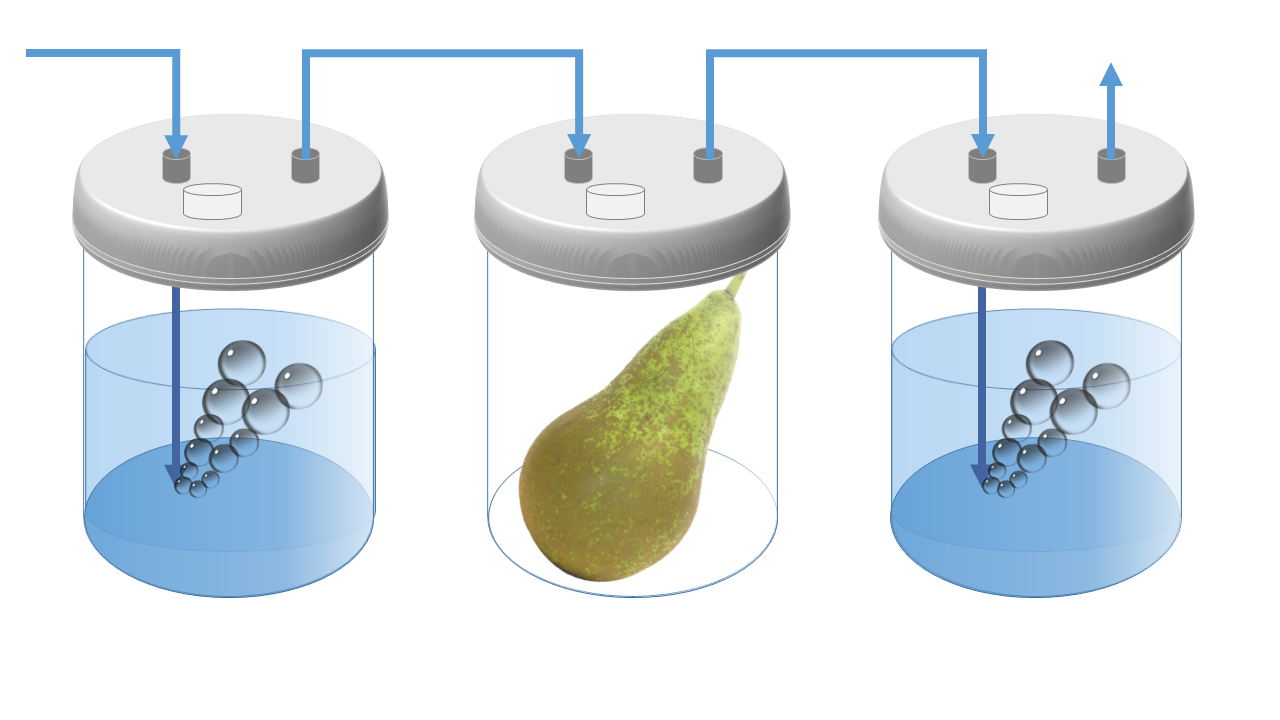
\includegraphics[width=0.8\textwidth]{figure/paper 1/pot.png}
	\caption{Graphical representation of the respiration jar measurement setup.}
	\label{figJar}
\end{figure}
\subsection{Optimal Experimental Design Methodology}
\label{Information}
Estimation of the parameter vector $\mathbf{p} = \begin{bmatrix}V_{\text{max}} & K_{\text{m}}\end{bmatrix}'$ was done by minimizing the squared error identification functional:
\begin{equation}
\mathbf{J} = \int_{0}^{t_\text{f}} (C(t) - C_\text{m}(\mathbf{p},Q(t),t))^2 \dd{t},
\label{J}
\end{equation}
where $t_\text{f}$ $[s]$ is the end time of the experiment. The functional $\mathbf{J}$ is often called the cost function.  This estimation problem was solved using the non-linear least squares algorithm, which required a starting value $\mathbf{p}^0$ for the parameters. Around that starting value, the model and $\mathbf{J}$ were linearized in the first iteration of the algorithm. When using that approach, the contours of $\mathbf{J}$ are ellipses, whose principal axes and surface area depend on the Fisher information matrix,
\begin{equation}
\mathbf{F} =  \int_{0}^{t_\text{f}}
\left(
\diff{C_\text{m}}{\mathbf{p}}
\right)'
\left(
\diff{C_\text{m}}{\mathbf{p}}
\right) \dd t,
\label{F}
\end{equation}
\parencite{fedorov}.The derivatives in this expression are generally referred to as parameter sensitivities:
\begin{equation}
\diff{C_\text{m}}{\mathbf{p}} =
\begin{bmatrix}
\dfrac{\partial C_\text{m}}{\partial V_{\text{max}}} & \dfrac{\partial C_\text{m}}{\partial K_{\text{m}}}
\end{bmatrix}.
\end{equation}
The larger the Fisher information matrix, the smaller the elliptic contours, and the steeper the cost functional $\mathbf{J}$ around its minimum, and thus the better the least squares identification problem is defined. The Fisher information matrix also has a second interpretation due to the fact that it is the inverse of the asymptotic variance covariance matrix of the best linear unbiased estimator (BLUE)  \parencite{munack1}. It summarizes the available information about the quality of the parameter estimates. The connection between the two interpretations of the Fisher information matrix is logical: the steeper the cost function, the better the least squares estimates fit the data compared to other parameter estimates. In that case, the quality of the estimates is large.
\\
\\
{\color{red}There exist more general definitions of the Fisher information matrix, which we use in subsequent chapters, in Sections \ref{secFIM2} and \ref{secFIM3}. The other definitions would lead to the same optimal respiration experiments presented in this chapter. However, the converse does not hold, the definition of the FIM in this chapter leads to different results in the other chapters.}
\\
\\
By modifying the input profile $Q(t)$, the magnitude of the Fisher information matrix, the steepness of the cost function and the surface areas of its contours can be optimized. To measure how large the Fisher information matrix is, different scalar functions of the Fisher information matrix have been proposed in the literature. These functions can be used to compare and score different experimental designs \parencite{atkinson1}. In this chapter, we used the determinant of the Fisher information matrix, $|\mathbf{F}|$, to compare different input profiles, which is referred to as the D-criterion. This criterion is inversely related to the area of the confidence ellipses of the parameter estimates, which should be minimal in an optimal experiment. Therefore, the optimized experimental design should maximize the determinant $|\mathbf{F}|$ over all admissible $\text{O}_2$ input profiles $Q(t)$:
\begin{equation}
\underset{\text{admissible Q(t)}}{\text{argmax}}|\mathbf{F}|.
\end{equation}
The parameter sensitivities $\dd C_\text{m}/\dd \mathbf{p}$ cannot be calculated analytically but have to be appended to the system of differential equations in equation (\ref{systemP1}), so they can be solved numerically. This is different from non-dynamical experiments, where analytical expressions exist for the sensitivities. The parameter sensitivity for the maximal respiration rate can be calculated from the following differential equation:
\begin{equation}
\diff{}{t}\left(\dfrac{\partial C_\text{m}}{\partial V_{\text{max}}}\right) = 
\dfrac{\partial}{\partial V_{\text{max}}}\left(\diff{C_\text{m}}{t}\right)
\label{sens1}
\end{equation}
\begin{equation*}
=
 -\frac{ 1}{V_\text{j}}Q(t)\dfrac{\partial C_\text{m}}{\partial V_{\text{max}}}  -
\end{equation*}
\begin{equation*}
\frac{ 1}{V_\text{j}}m_\text{p}\left(\frac{ \left( C_\text{m}(t) + V_{\text{max}}\dfrac{\partial C_\text{m}}{\partial V_{\text{max}}}\right)\left(K_\text{m} + C_\text{m}(t)\right) - \left(\dfrac{\partial C_\text{m}}{\partial V_{\text{max}}}V_{\text{max}}C_\text{m}(t)\right)}{(K_\text{m} + C_\text{m}(t))^2}	
\right).
\end{equation*}
The parameter sensitivity for the Michaelis-Menten constant  $\partial C_\text{m}/\partial K_{\text{m}}$ can be calculated in a similar manner:
\begin{equation}
\diff{}{t}\left(\dfrac{\partial C_\text{m}}{\partial K_{\text{m}}}\right) = 
\dfrac{\partial}{\partial K_{\text{m}}}\left(\diff{C_\text{m}}{t}\right)
\label{sens2}
\end{equation}
\begin{equation*}
=
\frac{ 1}{V_\text{j}} \left(-Q(t)\dfrac{\partial C_\text{m}}{\partial K_{\text{m}}} 
- m_\text{p}V_{\text{max}}\left(\frac{  \dfrac{\partial C_\text{m}}{\partial K_{\text{m}}}\left(K_\text{m} + C_\text{m}(t)\right) - \left(1 + \dfrac{\partial C_\text{m}}{\partial K_{\text{m}}}\right)C_\text{m}(t)}{(K_\text{m} + C_\text{m}(t))^2}
\right)\right).
\end{equation*}
In our search for optimal input profiles, we solved these differential equations using the Matlab implementation of the Dormand-Prince 45 method \parencite{matlab1}. Whenever the solver reached a discontinuity in the input profile, the solver was  terminated and restarted again with initial conditions equal to the previous final conditions. This prevent{ed} the adaptive time stepper from remaining stuck on the discontinuity. The integral in the expression of the Fisher information matrix $\mathbf{F}$ in equation (\ref{F}) and the squared error identification functional $\mathbf{J}$ in equation (\ref{J}) were  calculated using the trapezoid rule with the time points provided by the differential equation solver. 
\\
\\
The sensitivities in equations (\ref{sens1}) and (\ref{sens2}) and thus also the information matrix in equation (\ref{F}) depend on the unknown parameters $V_{\text{max}}$ and $K_{\text{m}}$. Therefore, we needed a starting parameter vector $\mathbf{p}^0$, to be able to calculate D-optimal designs. This technique is called locally optimal design, as the optimal designs obtained, are only truly optimal for the specific starting parameters in $\mathbf{p}^0$.
\subsection{Information Optimization}
\label{Optimization}
To search for an optimal experimental design, we first had to characterize the input profile $Q(t)$, to form a set of admissible input profiles. This method is called control vector parametrization in the optimal control theory literature \parencite{vassiliadis}. In that literature, methods for efficient numerical optimization of dynamic experiments were suggested as well, with a focus on continuous parameters \parencite{telen,bauer}. Our work is different in that we work with an integer parametrization of the input profile.
\\
\\
In this chapter, we focused on experiments lasting $24 \text{ h}$. The input $Q(t)$ could take $l$ equidistant different levels between a maximal input level, with a flow rate of $10 \text{ l/h}$, and a minimal input level, with zero flow rate. In Section \ref{Results}, we first consider examples with $l=2$. In these examples, only an on or off state was allowed. Next, we also consider a scenario with $l=11$, where the input could take $11$ values. The total time duration of the experiment was divided into $n$ equally long time-intervals. At the beginning of each of the $n$ intervals, the input could be changed from one input level to another. Note that this does not mean that the input had to be changed at these time points. We first consider a scenario in which the input could be changed every $2 \text{ h}$ ($n=12$). Next, we also consider a case where changes were allowed every $10 \text{ min}$ ($n=144$).
\\
\\
Because a full enumeration of the design space is not feasible for larger values of $n$ and $j$, a numerical routine had to be used to optimize the experiment. Popular choices in design of experiments are variants of the coordinate-exchange algorithm \parencite{meyer}. Therefore, we have also used a coordinate-exchange algorithm. In its simplest variant, similar to the one described in \textcite{goos1}, a random feasible starting design was generated first. Next, the most informative of the possible input levels during the first of the $n$ time-intervals was identified by comparing all $l-1$ alternatives to the original. If the best of the alternative levels led to a more informative experiment, the change was accepted. Otherwise, the previous input profile was reinstated. Subsequently, the same kind of change was evaluated for the next time-interval. When all $n$ intervals had been considered, the algorithm evaluated the first time-interval again. This procedure was continued until no more improvements could be made to the design, in a whole pass through the entire set of $n$ time points. This optimization was performed $m$ times, where $m$ is a specified number of iterations. The best of the $m$ results was selected as the optimal input profile. Pseudo-code for this algorithm is shown in Figure \ref{pseudo1}. 
\begin{figure}
	
	\begin{algorithm}[H]
		optimal profile = random feasible design\;
		\For{iteration = $1$ to $m$}{
			generate random feasible design\;
			improvement = yes\;
			\While{improvement == yes}{
				improvement = no\;
				\For{$k = 1$ to $n$}{
					information = information of current profile\;
					\For{$j = 1$ to $l-1$ other levels  in interval $k$}{
						switch input of $k$th time-interval to $j$th other level\;
						new information = information of the resulting profile\;
						\If{new information > information}			{
							accept change\;
							information = new information\;
							improvement = yes\;
						}
					}
				}
			}
			\If{information $m$th input profile > information optimal profile}	{
				optimal profile = $m$th input profile	
			}
		}
		
	\end{algorithm}
	
	\caption{Initial coordinate-exchange algorithm.}
	\label{pseudo1}
\end{figure}
\\
\\
When changing the input at a certain time $t'$, the output $C_m(t)$ for all $t\geq t'$ is affected. This distinguishes dynamic experiments from static experiments. Due to this feature, running through the $n$ time-intervals in order might lead the coordinate-exchange algorithm to get stuck in a local minimum. Because our initial coordinate-exchange algorithm indeed did get stuck in the same local optima quite often, as shown in the examples in Section \ref{Results}, we propose a variant of the coordinate-exchange algorithm in which the optimization does not start with the first time-interval and subsequently moves to the next interval, but picks the $n$ intervals in a random order, without repetition. This procedure is repeated until no more improvements can be made. Pseudo-code of this modified coordinate-exchange algorithm is shown in Figure \ref{pseudo2}.
\begin{figure}
	\begin{algorithm}[H]
		optimal profile = random feasible design\;
		\For{iteration = $1$ to $m$}{
			generate random feasible design\;
			improvement = yes\;
			\While{improvement == yes}{
				improvement = no\;
				$S = \{1,2,...,n\}$\;
				\For{$i = 1$ to $n$}{
					$k$ = randomly selected element of $S$\;
					information = information of current profile\;
					\For{$j = 1$ to $l-1$ other levels in interval $k$}{
						switch input of $k$th time-interval to $j$th other level\;
						new information = information of the new profile\;
						\If{new information > information}			{
							accept change\;
							information = new information\;
							improvement = yes\;
						}
					}
				}
				remove $k$ from $S$
			}
			\If{information $m$th input profile > information optimal profile}	{
				optimal profile = $m$th input profile	
			}
		}
	\end{algorithm}
	\caption{Modified coordinate-exchange algorithm.}
	\label{pseudo2}
\end{figure}
\section{Results}
\label{Results}
In this section, we report results concerning three different optimal experimental designs we constructed, each with their own parametrization of the input profile. We start with a proof of concept example, where the input could only take two levels (on/off) and the level can be changed every $2 \text{ h}$. The resulting optimal experimental  design is compared to several intuitive benchmarks. Next, we explain how we refined the design space of our experiment in two different manners to study the resulting increase in information. We first subdivide every time-interval of $2 \text{ h}$ into 12 intervals of $10 \text{ min}$ each. Second, we allowed 11 different input levels.
\\
\\
As initial parameter vector $\mathbf{p}^0$ for all our computations, we used the respiration parameter estimates for Conference pear, as reported by \textcite{lammertyn1}. More specifically, we used a maximal respiration rate, $V_{\text{max}}$, of $0.2324 \text{ mmol kg}^{-1}\text{s}^{-1}$, calculated at a temperature of $20$ $^\circ C$, and the value $5.9$ $\%$ for the Michaelis-Menten constant $K_m$. {\color{red}Concentrations in volume percentages are calculated by assuming atmospheric pressure in the jar, and applying the ideal gas law.}
\subsection{Proof of Concept Example}
\label{Experiment1}
\subsubsection{Optimal design}
The optimal experimental design depicted in Figure \ref{input1} was found after an exhaustive search over all $2^{12}$ possible input profiles. The optimal input is a pulse and only pumps air into the jar during a single time-interval, from $6 \text{ until } 8 \text{ h}$. The corresponding simulated output, the $\text{O}_2$ concentration $C(t)$ is depicted in Figure \ref{output1}. The D-criterion value for the optimal design equals $3.56\e{15}$. No alternative optima with the same information content were found. Why this input profile is optimal can be intuitively explained by the concentration in the jar near the end of the experiment. That concentration is roughly equal to the Michaelis-Menten constant $K_m$, which determines the switching behavior between the linear and saturated part of the Michaelis-Menten curve. Measuring in this concentration range provides information about this parameter. If the two-hour interval in which air is pumped into the jar would have started earlier, the concentration in the jar at the end of the experiment would have dropped even lower, and the information content of the experiment would decrease. This is due to the fact that, in our model, which neglects fermentation, a very low $\text{O}_2$ concentration means almost no respiration, and thus little information about respiration parameters. Conversely, if the two-hour interval would start later, little information about the switching behavior would be gained.
\begin{figure}
	\centering
	\begin{subfigure}[b]{0.45\textwidth}
		%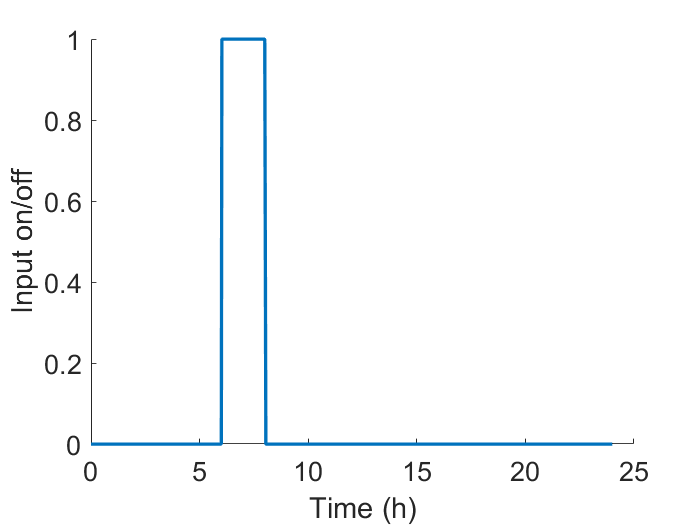
\includegraphics[width=\textwidth]{figure/paper 1/input.png}
		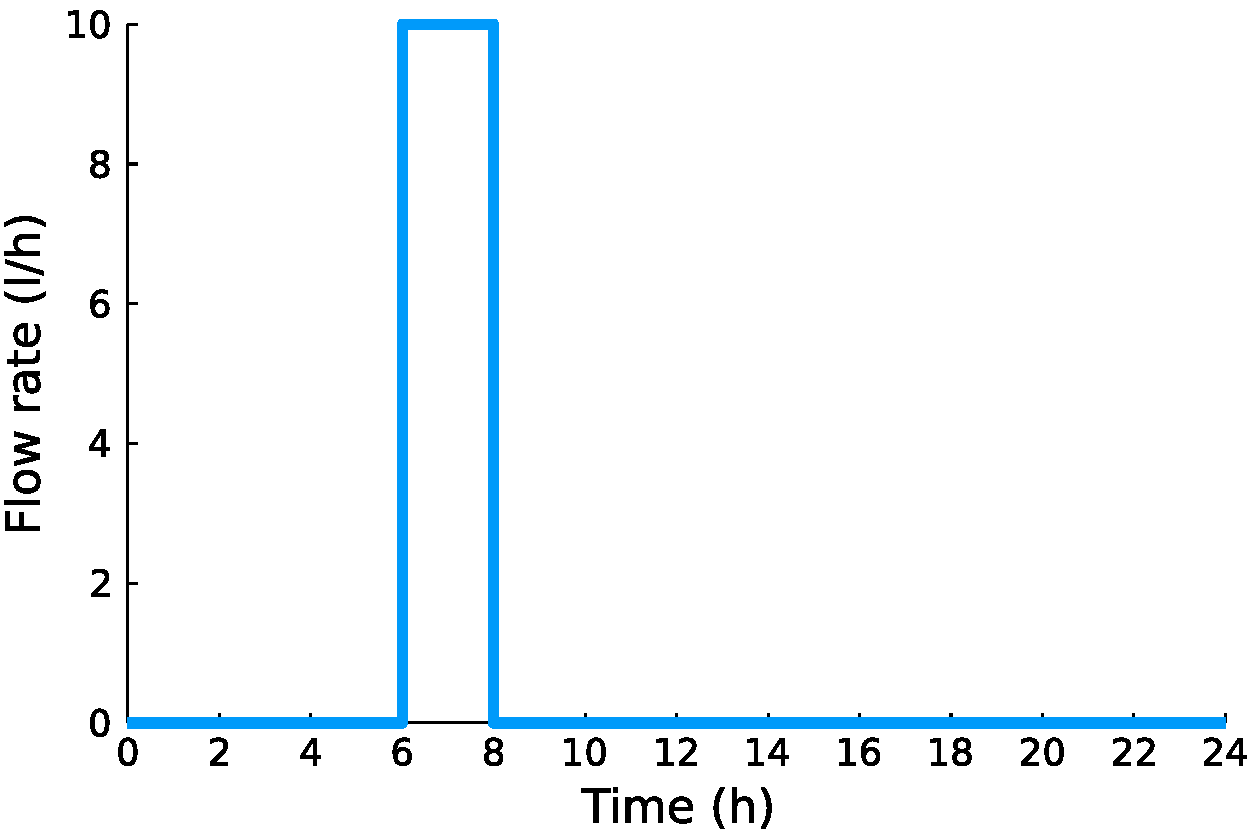
\includegraphics[width=\textwidth]{figure/paper 1/extra1}
		\caption{Optimal $\text{O}_2$ input profile.}
		\label{input1}
	\end{subfigure}
	~ %add desired spacing between images, e. g. ~, \quad, \qquad, \hfill etc. 
	%(or a blank line to force the subfigure onto a new line)
	\begin{subfigure}[b]{0.45\textwidth}
		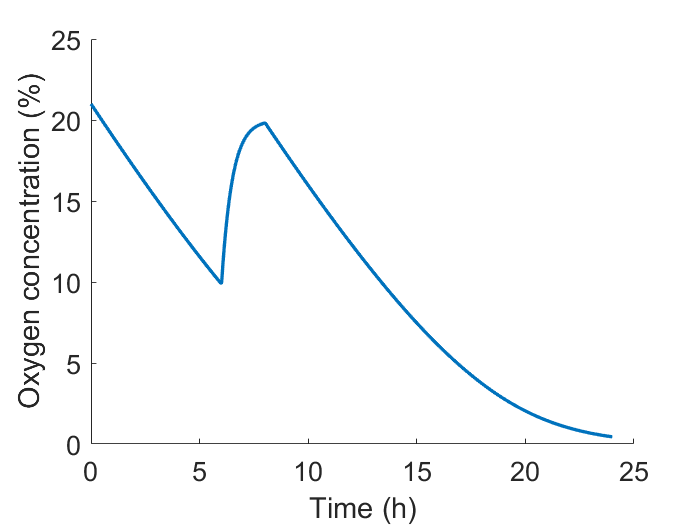
\includegraphics[width=\textwidth]{figure/paper 1/design.png}
		\caption{$\text{O}_2$ concentration in the jar.}
		\label{output1}
	\end{subfigure}
	\caption{Optimal design, assuming $l=2$ and $n=12$: pulse input after $6 \text{ h}$.}
	\label{figODE1}
\end{figure}
\begin{figure}
	\centering
	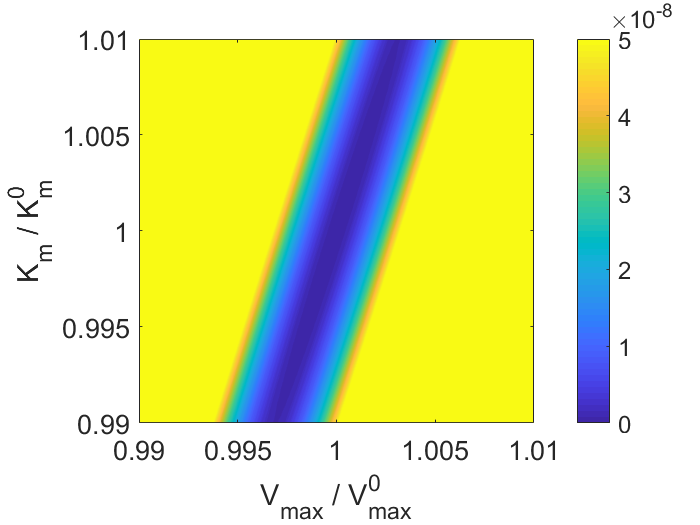
\includegraphics[width=0.8\textwidth]{figure/paper 1/compare1.png}
	\caption{SSE contours for the optimal design in Figure \ref{input1}.}
	\label{figCompare1}
\end{figure}
\\
\\
While a full enumeration of the design space was feasible for our proof of concept example, we also tested the performance of the initial and the modified coordinate-exchange algorithm. In each case, we ran the algorithm $10,000$ times. When applying the initial algorithm, the optimal experiment was found only ten times. So, while this simple algorithm performs well for response surface models, it is clearly not appropriate for our dynamical models, with our specific parametrization of the $\text{O}_2$ input profile. When applying the modified algorithm, we obtained the global optimum in $1,014$ of the $10,000$ iterations of the algorithm, a considerable improvement.
\subsubsection{Comparison to benchmark designs}
We now compare the first optimal experimental design of Figure \ref{input1} to four intuitive benchmark designs, also considered in the full enumerative search. More specifically, we provide a comparison with two constant input profiles, a maximally dynamic profile and an alternative pulse. Table \ref{table1} lists these benchmark designs and their D-criterion values.
\begin{table}
	\centering
	\begin{tabular}{|c|c|}
		\hline 
		Experimental design & D-criterion \\ 
		\hline 
		Optimal design: pulse after $6 \text{ h}$& $3.56\e{15}$  \\ 
		
		Alternative design: Always on & $9.37\e{7}$ \\ 
		
		Alternative design: Always off & $2.66\e{15}$ \\ 
		
		Alternative design: Switching on/off & $2.64\e{11}$ \\ 
		
		Alternative design: pulse after $4 \text{ h}$ & 
		$3.16\e{15}$ \\ 
		\hline
	\end{tabular} 
	\caption{D-criterion values for both the optimal design as well as several benchmarks, assuming $l=2$ and $n=12$. {\color{red}These designs are shown in Figures \ref{figODE1} --- \ref{compare4}.}} 
	\label{table1}
\end{table}
\\
\\
We also performed a detailed graphical comparison by calculating the squared error identification functional in Equation (\ref{F}) for different parameter vectors, in the neighborhood of the initial parameter vector $\mathbf{p}^0$. If other parameters would fit the system almost equally well, the sum of squared errors (SSE) would not vary substantially in the neighborhood of the initial parameters values, suggesting imprecise parameter estimation. The SSE contours resulting from the first optimal experimental design are shown in Figure \ref{figCompare1}. All values larger than the maximum on the color bar are displayed in the same yellow color as the maximum itself. The values on the axes are relative to the initial parameter values. The function is steep in the vertical and horizontal direction, indicating precise parameter estimates. However, the principal axes of the ellipses are not parallel with the horizontal and vertical axes, and the contours are elongated diagonally. This indicates that even the optimal experimental design would result in correlated parameter estimates. In other words, the two parameters cannot be estimated independently. This is a well-known problem when estimating Michaelis-Menten models.
\\
\\
Figure \ref{SSEcompare2} depicts the SSE contours resulting from the constant input profile that continuously pumps air into the jar, for the full duration of the experiment in Figure \ref{inputcompare2}. The D-criterion corresponding to that experimental design is much lower, $9.37\e{7}$. As a result, this benchmark experiment performs considerably worse in terms of the quality of the estimates than the optimal design in Figure \ref{figODE1}: the SSE value is insensitive to the values of the parameters $K_\text{m}$ and $V_{\text{max}}$.
\\
\\
The other constant input profile we considered as a benchmark and which is shown in Figure \ref{inputcompareLiterature}, is the always off profile. This profile has a D-criterion value much closer to that of the optimal design, namely $2.66\e{15}$. The resulting contours for the SSE value are shown in Figure \ref{SSEcompareLiterature}, and resemble those in Figure \ref{figCompare1}. However, they have a slightly larger surface area.
\\
\\
Figure \ref{compare3} demonstrates that the SSE contours produced by a maximally dynamic input profile are quite different from the contours produced by the optimal design. The maximally dynamic profile switches input every $2 \text{ h}$ and the D-criterion value equals $2.64\e{11}$, for that profile. This demonstrates that optimal dynamic design of experiments is not equivalent to changing the input as frequently as possible.
\\
\\
In Figure \ref{compare4}, we show a pulse input function that occurs $2 \text{ h}$ earlier than the pulse in the optimal experimental design, as well as the SSE contours corresponding to that input. This profile performs much better than the other benchmark experimental designs. This is also reflected in the D-criterion value of $3.16\e{15}$, which shows that designs that are close to the optimal design are also similar in information content.
\begin{figure}[H]
	\centering
	\begin{subfigure}[b]{0.45\textwidth}
		%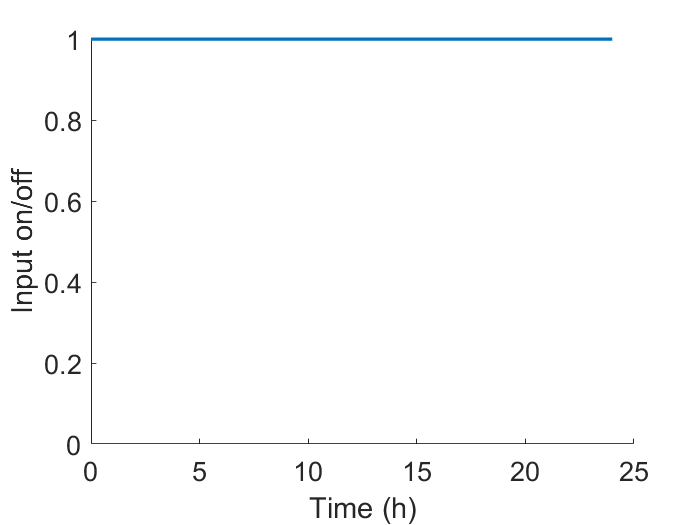
\includegraphics[width=\textwidth]{figure/paper 1/compare2input.png}
		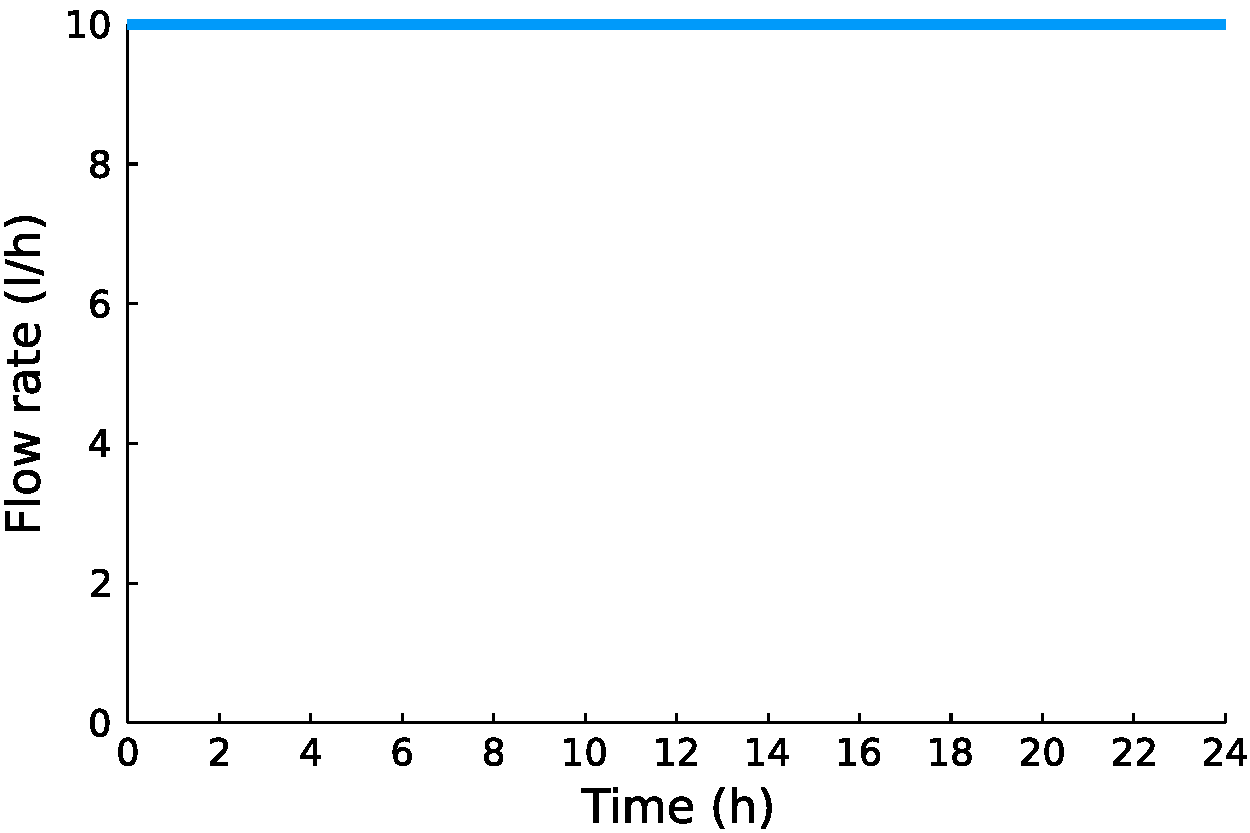
\includegraphics[width=\textwidth]{figure/paper 1/extra2}
		\caption{Oxygen input profile.}
		\label{inputcompare2}
	\end{subfigure}
	~ %add desired spacing between images, e. g. ~, \quad, \qquad, \hfill etc. 
	%(or a blank line to force the subfigure onto a new line)
	\begin{subfigure}[b]{0.45\textwidth}
		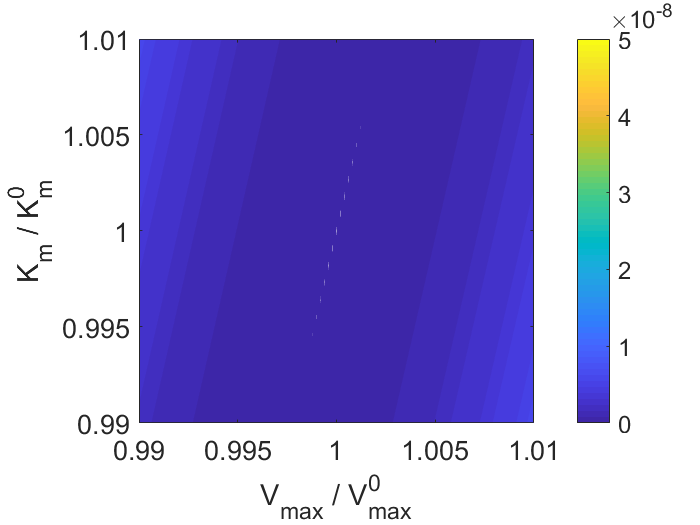
\includegraphics[width=\textwidth]{figure/paper 1/compare2.png}
		\caption{SSE contours.}
		\label{SSEcompare2}
	\end{subfigure}
	\caption{First benchmark: an always-on input profile.}
	\label{compare2}
\end{figure}
\begin{figure}[H]
	\centering
	\begin{subfigure}[b]{0.45\textwidth}
		%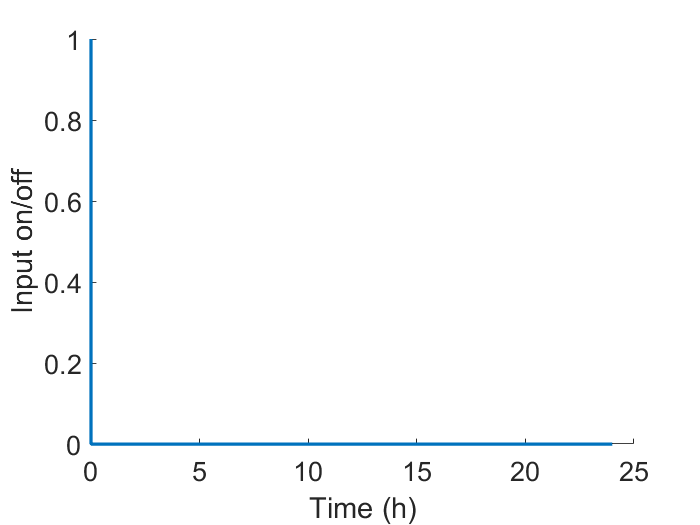
\includegraphics[width=\textwidth]{figure/paper 1/inputLiterature.png}
		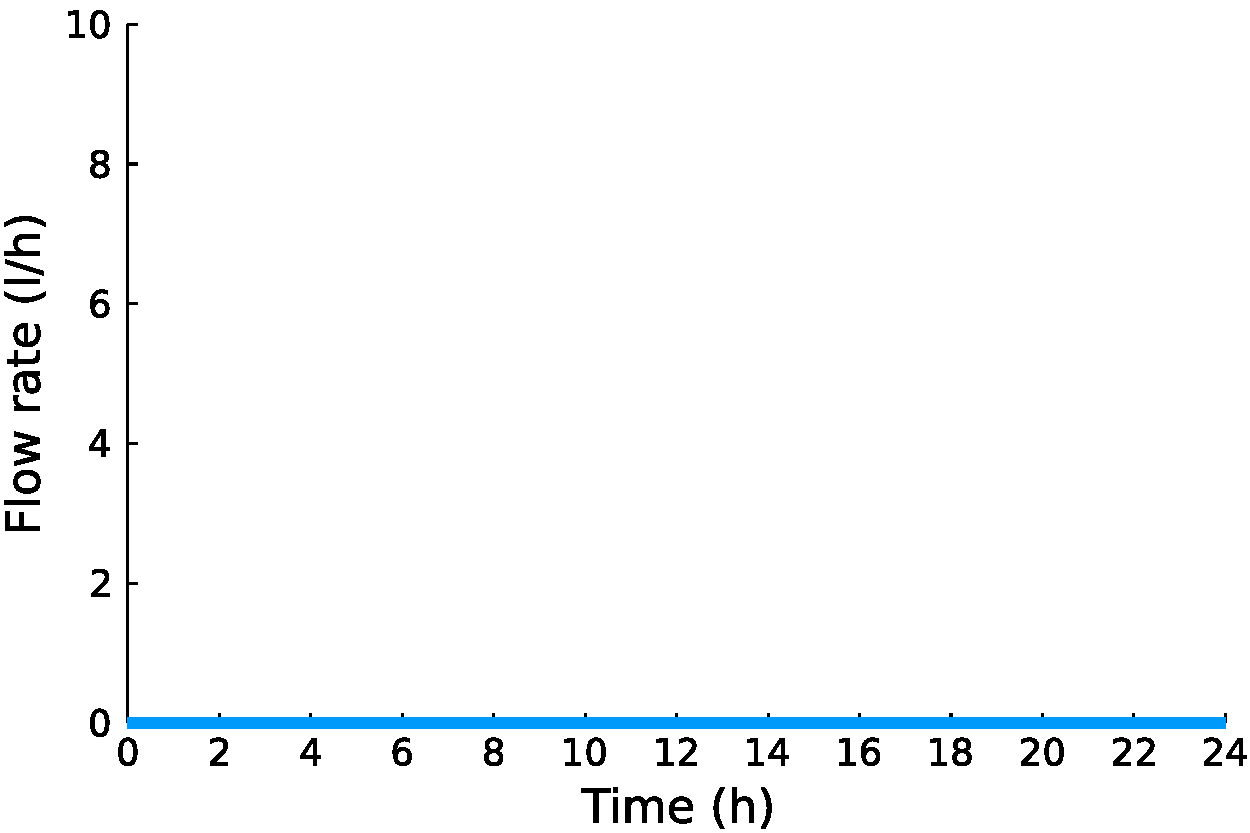
\includegraphics[width=\textwidth]{figure/paper 1/extra3}
		\caption{Oxygen input profile.}
		\label{inputcompareLiterature}
	\end{subfigure}
	~ %add desired spacing between images, e. g. ~, \quad, \qquad, \hfill etc. 
	%(or a blank line to force the subfigure onto a new line)
	\begin{subfigure}[b]{0.45\textwidth}
		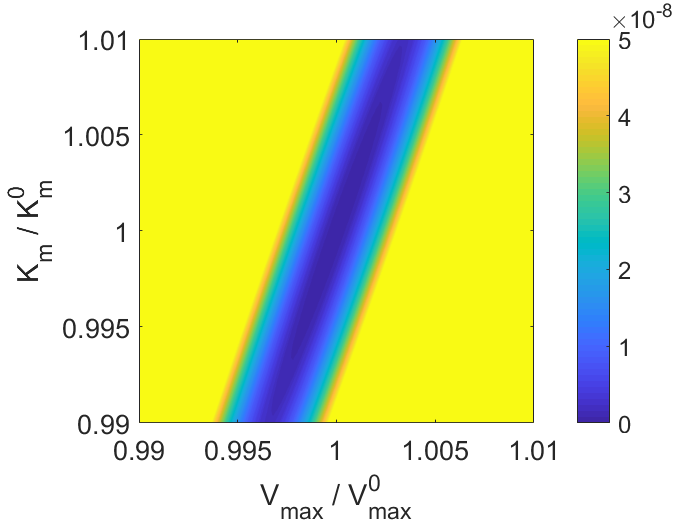
\includegraphics[width=\textwidth]{figure/paper 1/compareLiterature.png}
		\caption{SSE contours.}
		\label{SSEcompareLiterature}
	\end{subfigure}
	\caption{Second benchmark: an always-off input profile.}
	\label{compareLiterature}
\end{figure}
\begin{figure}[H]
	\centering
	\begin{subfigure}[b]{0.45\textwidth}
		%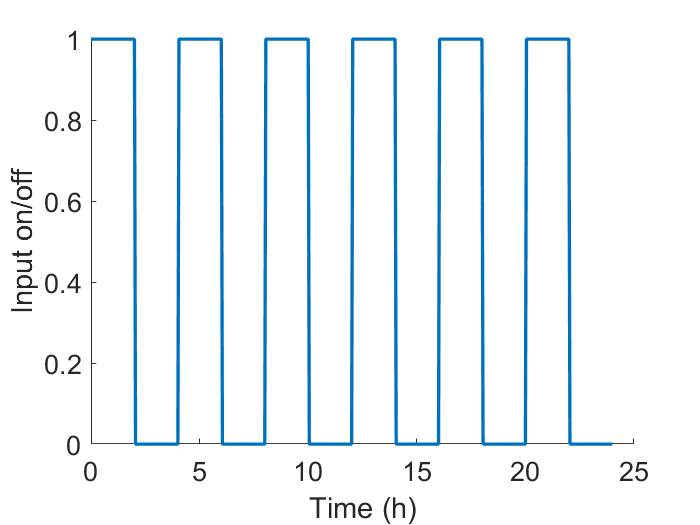
\includegraphics[width=\textwidth]{figure/paper 1/compare3input.png}
		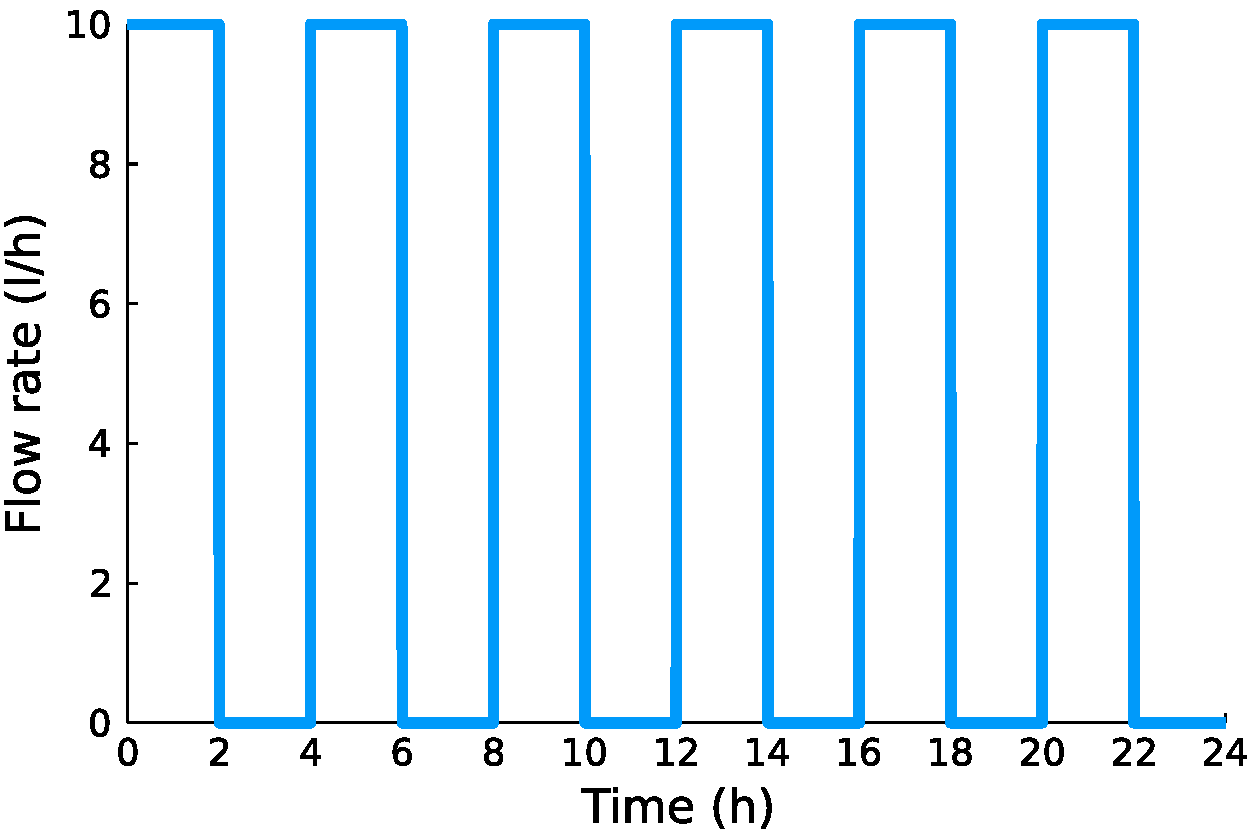
\includegraphics[width=\textwidth]{figure/paper 1/extra4}
		\caption{Oxygen input profile.}
		\label{inputcompare3}
	\end{subfigure}
	~ %add desired spacing between images, e. g. ~, \quad, \qquad, \hfill etc. 
	%(or a blank line to force the subfigure onto a new line)
	\begin{subfigure}[b]{0.45\textwidth}
		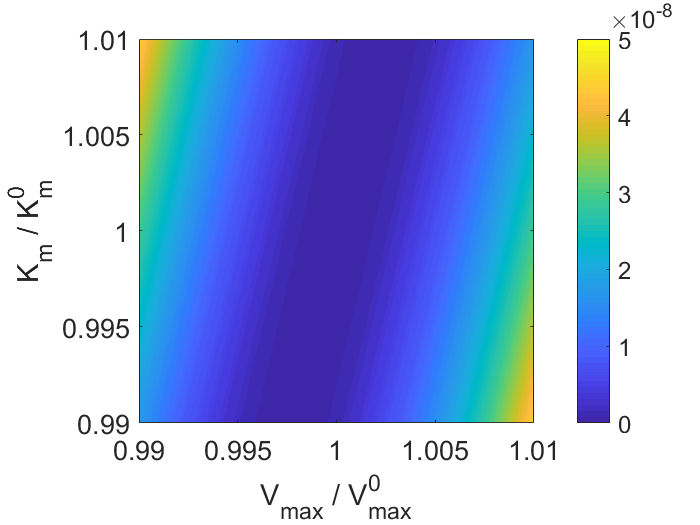
\includegraphics[width=\textwidth]{figure/paper 1/compare3.png}
		\caption{SSE contours.}
		\label{SSEcompare3}
	\end{subfigure}
	\caption{Third benchmark: a constantly switching input profile.}
	\label{compare3}
\end{figure}
\begin{figure}[H]
	\centering
	\begin{subfigure}[b]{0.45\textwidth}
		%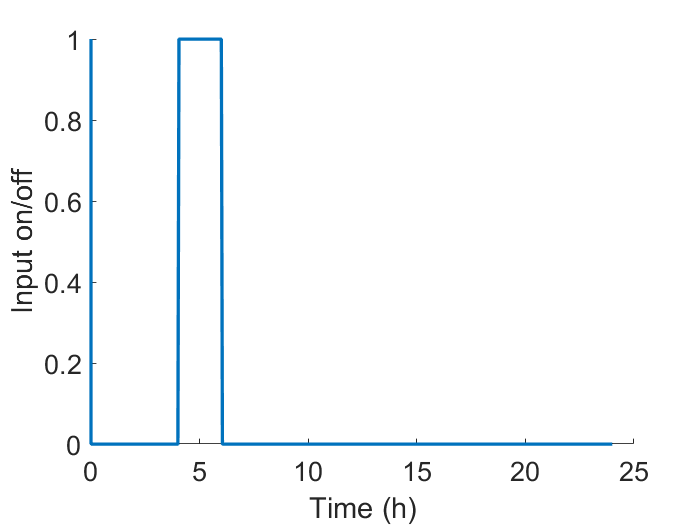
\includegraphics[width=\textwidth]{figure/paper 1/compare4input.png}
		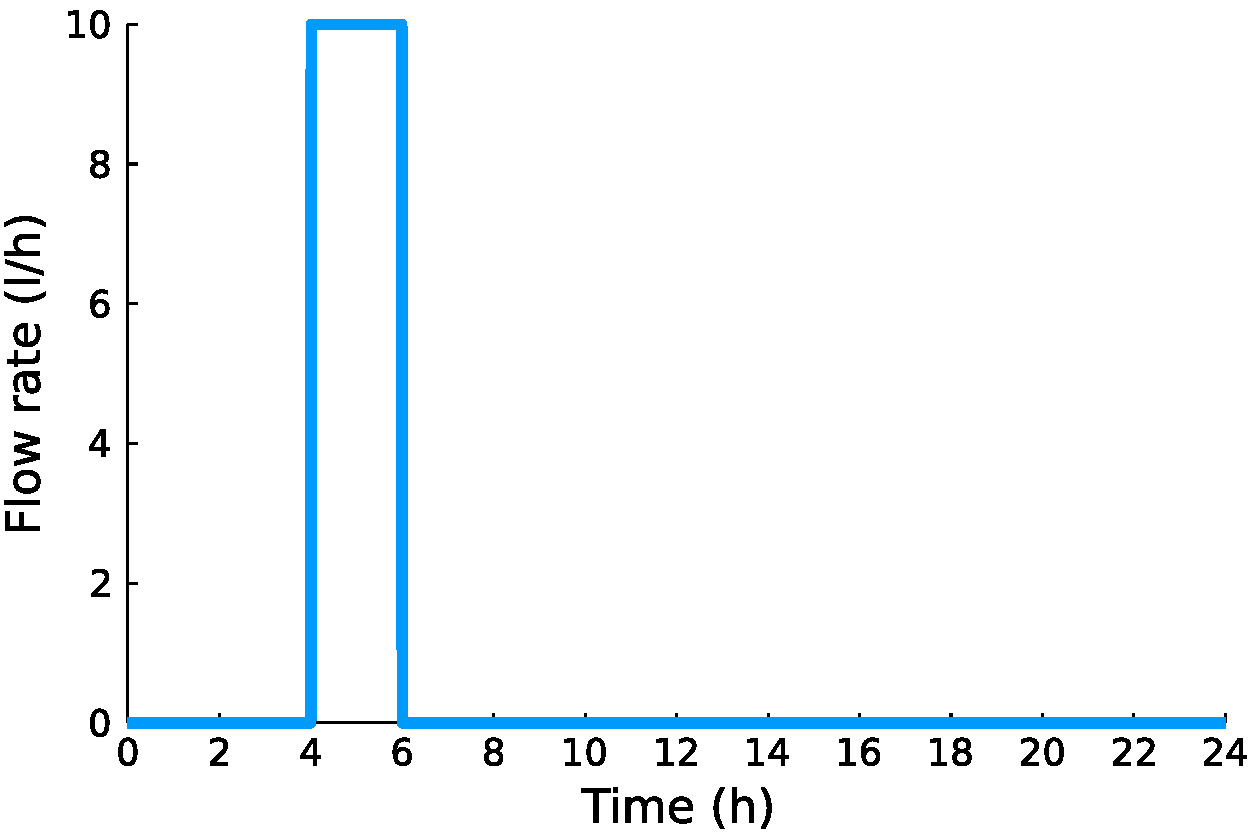
\includegraphics[width=\textwidth]{figure/paper 1/extra5}
		\caption{Oxygen input profile.}
		\label{inputcompare4}
	\end{subfigure}
	~ %add desired spacing between images, e. g. ~, \quad, \qquad, \hfill etc. 
	%(or a blank line to force the subfigure onto a new line)
	\begin{subfigure}[b]{0.45\textwidth}
		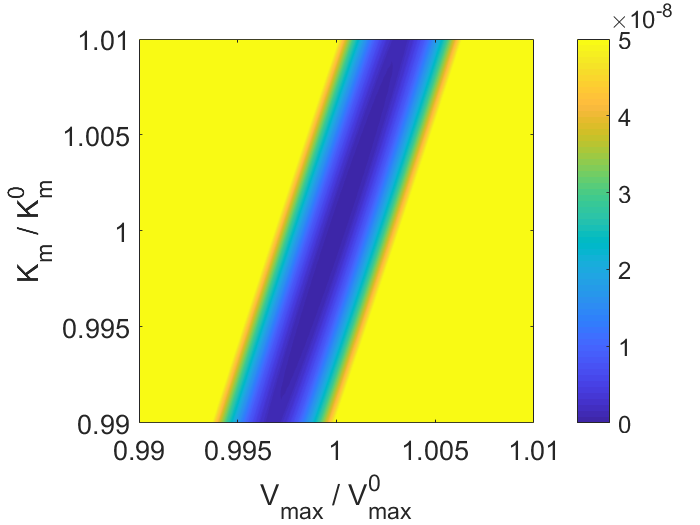
\includegraphics[width=\textwidth]{figure/paper 1/compare4.png}
		\caption{SSE contours}
		\label{SSEcompare4}
	\end{subfigure}
	\caption{Fourth benchmark: pulse input after $4 \text{ h}$.}
	\label{compare4}
\end{figure}
\subsection{Refining the Design Space}
We refined the parametrization of the proof of concept experimental designs in two different ways. The D-criterion values of the optimal input profiles are listed in Table \ref{table2}.
\label{Refinement}
\begin{table}
	\centering
	\begin{tabular}{|c|c|}
		\hline 
		Optimal experimental design & D-criterion \\ 
		\hline 
		$n = 12$ and $l = 2$& $3.56\e{15}$  \\ 
		
		$n = 144$ and $l = 2$& {\color{red}$5.15\e{17}$ }\\ 
		
		$n = 12$ and $l= 11$& {\color{red}$5.13\e{17}$} \\ 
		\hline
	\end{tabular} 
	\caption{D-criterion values for optimal experimental designs with different parametrizations  in Sections \ref{Experiment2} and \ref{Experiment3}. {\color{red}These designs are shown in Figures \ref{figODE1}, \ref{figODE2} and \ref{figODE3}.}} 
	\label{table2}
\end{table}

\subsubsection{Allowing more frequent input changes}
\label{Experiment2}
For the construction of our second optimal experimental design, we allowed the inputs to be changed every $10 \text{ min}$, instead of every $2 \text{ h}$, while still only allowing an on or off input. As all admissible input profiles from the proof of concept example are also admissible under the new settings, the second optimal design problem generalizes the initial one, since $120 \text{ min}$ is divisible by $10 \text{ min}$. The set of admissible input profiles in our second optimal design problem can thus be considered as a refinement of the first. To identify the optimal experimental design for the new problem, we used $10, 000$ iterations of the modified coordinate-exchange algorithm. The unique best design found by the modified coordinate-exchange algorithm is depicted in Figure \ref{input2}. It was found in 45 of the $10, 000$ iterations of the algorithm and involves two short $10 \text{ min}$ pulses during the second half of the experiment. The resulting $\text{O}_2$ concentration in the jar is shown in Figure \ref{output2}. The D-criterion value of this design amounts to {\color{red}$5.15\e{17}$}, which is much better than the value of the optimal design in the proof of concept example.
\begin{figure}
	\centering
	\begin{subfigure}[b]{0.45\textwidth}
		%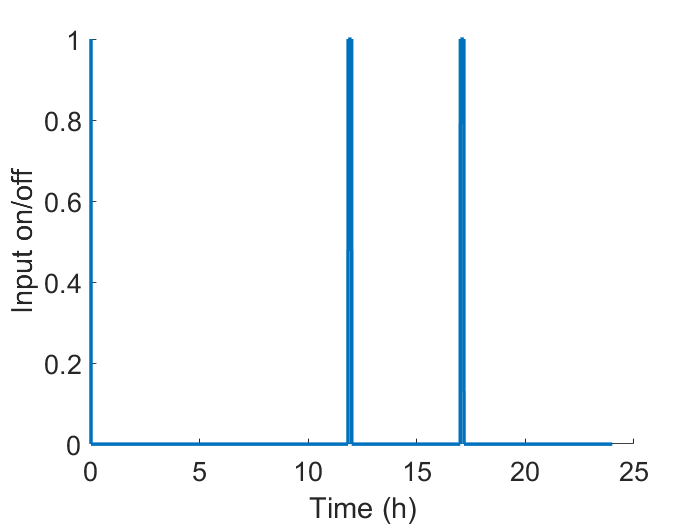
\includegraphics[width=\textwidth]{figure/paper 1/input2.png}
		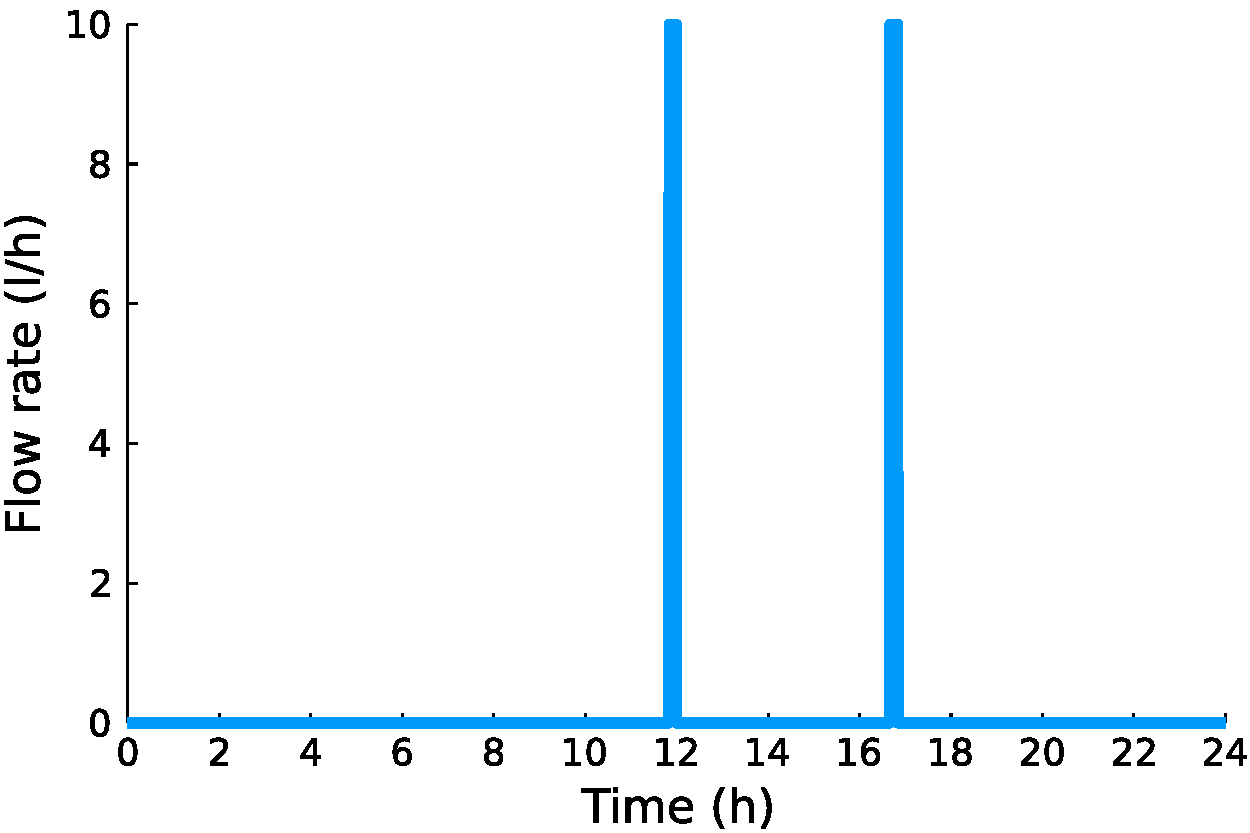
\includegraphics[width=\textwidth]{figure/paper 1/extra6}
		\caption{$\text{O}_2$ input profile.}
		\label{input2}
	\end{subfigure}
	~ %add desired spacing between images, e. g. ~, \quad, \qquad, \hfill etc. 
	%(or a blank line to force the subfigure onto a new line)
	\begin{subfigure}[b]{0.45\textwidth}
		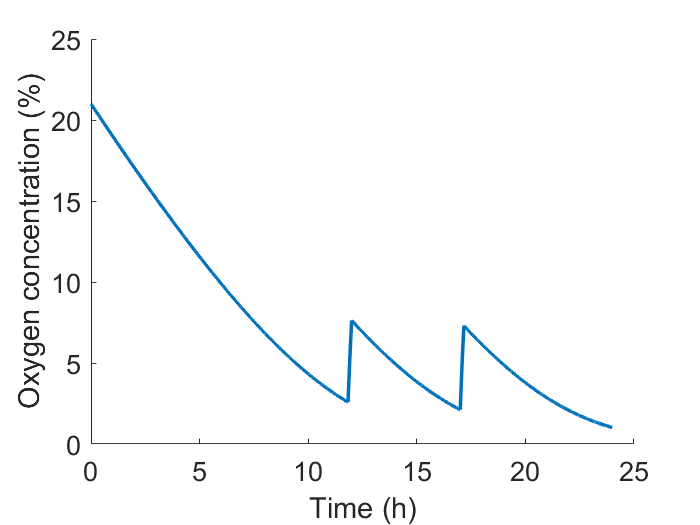
\includegraphics[width=\textwidth]{figure/paper 1/design2.png}
		\caption{$\text{O}_2$ concentration in the jar.}
		\label{output2}
	\end{subfigure}
	\caption{Optimal design, assuming $l=2$ and $n=144$: two short pulses during the second half of the experiment.}
	\label{figODE2}
\end{figure}
\\
\\
The new optimal profile differs substantially from the first in Figure \ref{input1}: instead of one longer pulse from $6 \text{ to } 8 \text{ h}$, two shorter $10 \text{ min}$ pulses after $12 \text{ and } 17 \text{ h}$ are preferred. The reason why this design is optimal is, however, very similar to that of the previous example. After an initial decrease, the $\text{O}_2$ concentration in the jar keeps hovering around the value of the Michaelis-Menten constant $K_\text{m}$, providing information about the switching behavior of the system between saturated and linear respiration. If the $\text{O}_2$ concentration would drop even lower, little respiration would occur and thus little information would be gained concerning the two model parameters. The preference for two short pulses over one longer pulse can be explained by comparing Figure \ref{figODE2} to Figure \ref{output1}. A longer pulse increases the $\text{O}_2$ concentration in the jar almost to the initial one. Since the system always starts at atmospheric conditions, information about maximal respiration is always present in the initial phase of the experiment. Returning to that high concentration does not yield new information. Instead, there is added value in studying the respiration at concentrations around $K_\text{m}$. Therefore, the optimal profile involving two shorter pulses focuses more on the switching behavior instead of revisiting the region of saturated respiration.
\subsubsection{Allowing more input levels}
\label{Experiment3}
In our final optimization, we allowed the input to take 11 different levels, equally spaced between the maximum and minimum input level. The input was only allowed to be changed every $2 \text{ h}$, unlike in the previous example. Again, all possible designs encountered during the first optimization, were considered in this third optimization problem. So, this example also generalizes the proof of concept example. The unique best design found using $10,000$ iterations of the modified coordinate-exchange algorithm, is depicted in Figure \ref{input3}. That input profile was found in 75 of the 10,000 iterations. The corresponding $\text{O}_2$ concentration in the jar is shown in Figure \ref{output3}. The D-criterion value of {\color{red}$5.13\e{17}$} is very similar to that of the input profile in Figure \ref{input2}, as can be seen in Table \ref{table2}.
\begin{figure}
	\centering
	\begin{subfigure}[b]{0.45\textwidth}
		%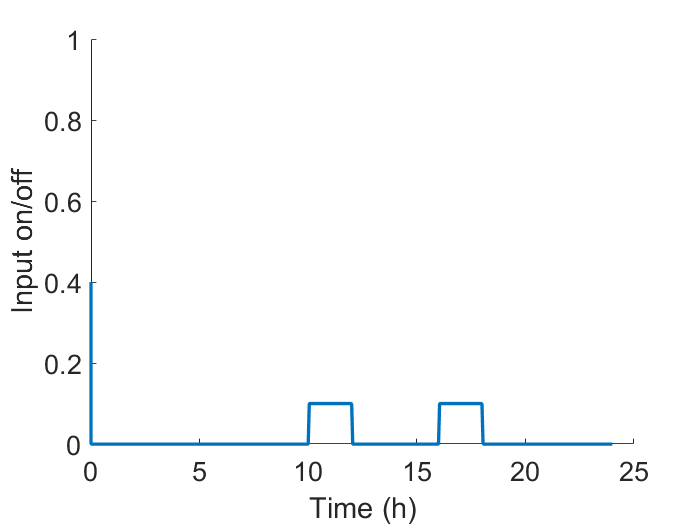
\includegraphics[width=\textwidth]{figure/paper 1/input3.png}
		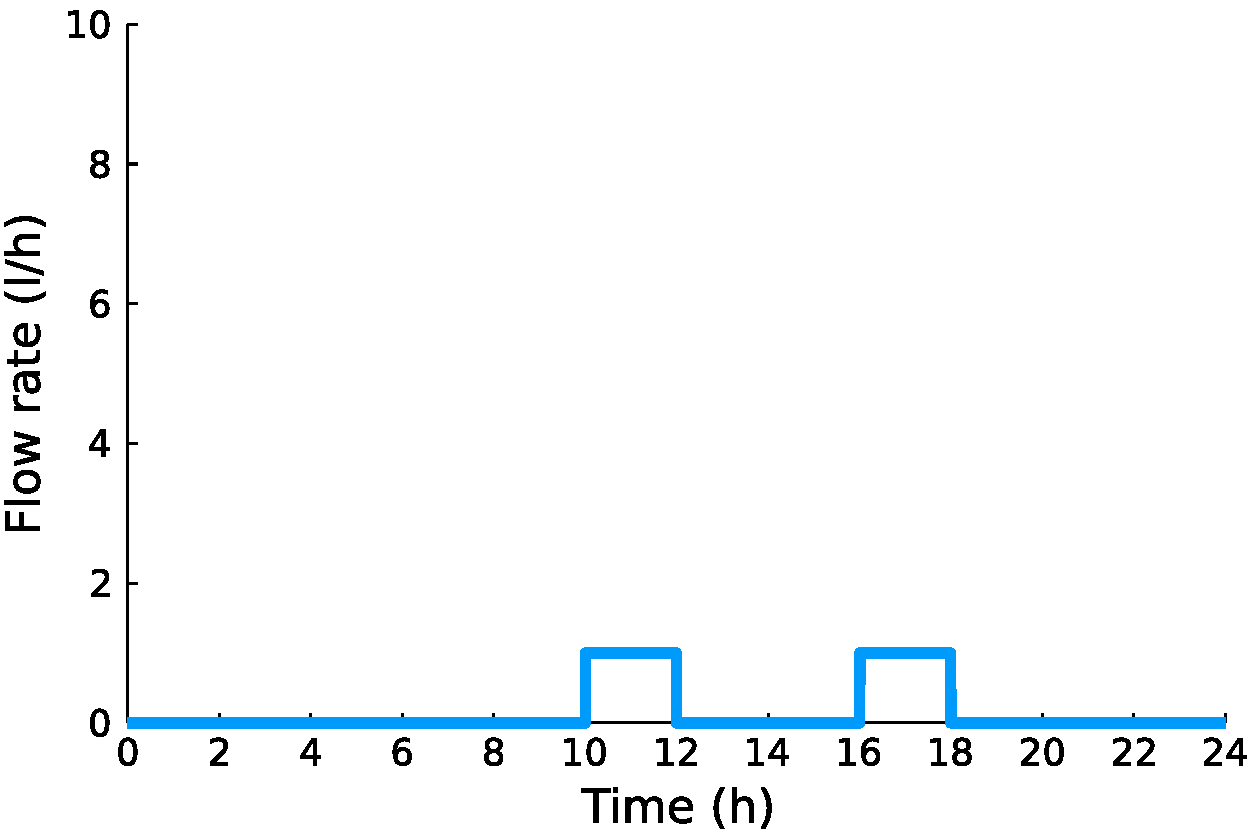
\includegraphics[width=\textwidth]{figure/paper 1/extra7}
		\caption{Optimal $\text{O}_2$ input profile.}
		\label{input3}
	\end{subfigure}
	~ %add desired spacing between images, e. g. ~, \quad, \qquad, \hfill etc. 
	%(or a blank line to force the subfigure onto a new line)
	\begin{subfigure}[b]{0.45\textwidth}
		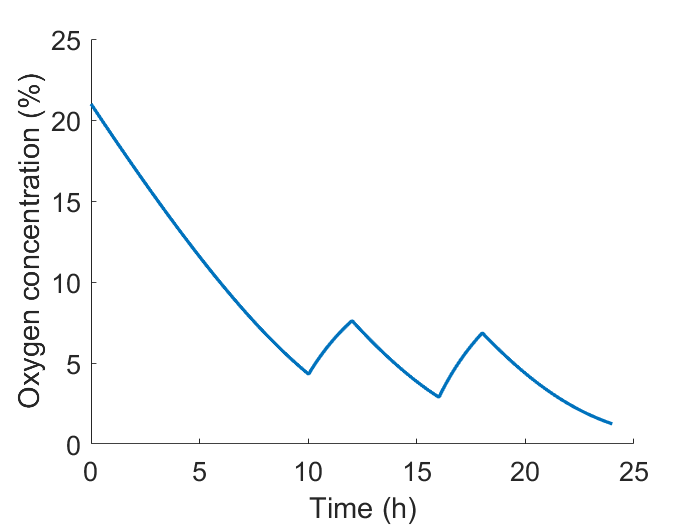
\includegraphics[width=\textwidth]{figure/paper 1/design3.png}
		\caption{$\text{O}_2$ concentration in the jar.}
		\label{output3}
	\end{subfigure}
	\caption{Optimal design, assuming $l = 11$ and $n = 12$: two small pulses after $10 \text{ h}$ and $16 \text{ h}$.}
	\label{figODE3}
\end{figure}
\\
\\
A similar dynamic input, consisting of two pulses, seems to be preferred in the last two examples. In the third, experiment the small pulses take the minimum non-zero input value of $0.1$, or $10$ $\%$ of the maximum allowed flow rate. The simulated outlet $\text{O}_2$ concentrations shown on Figure\ref{output2} and Figure \ref{output3}, look remarkably similar, which shows that even with different parametrizations of the input curve, a similar dynamic behavior can be achieved.
\\
\\
The SSE contours in Figure \ref{figCompare5} correspond to the input profiles of Figure \ref{input2} and Figure \ref{input3}. As already noted, the designs involve similar dynamic $\text{O}_2$ concentration trends, have similar D-criterion values and thus also have very similar contour plots. The contours in Figure \ref{figCompare5} are also much steeper than those in Figure \ref{figCompare1}, but they are still elongated diagonally. So, even a refinement of the design space did not help to remove the correlation between the two parameter estimates.
\begin{figure}
	\centering
	\begin{subfigure}[b]{0.45\textwidth}
		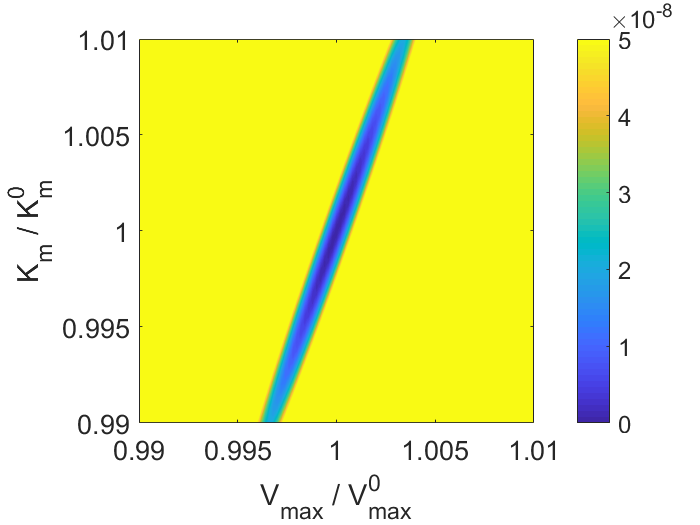
\includegraphics[width=\textwidth]{figure/paper 1/compare5.png}
		\caption{Optimal design in Figure \ref{input2}.}
		\label{SSEopt2}
	\end{subfigure}
	~ %add desired spacing between images, e. g. ~, \quad, \qquad, \hfill etc. 
	%(or a blank line to force the subfigure onto a new line)
	\begin{subfigure}[b]{0.45\textwidth}
		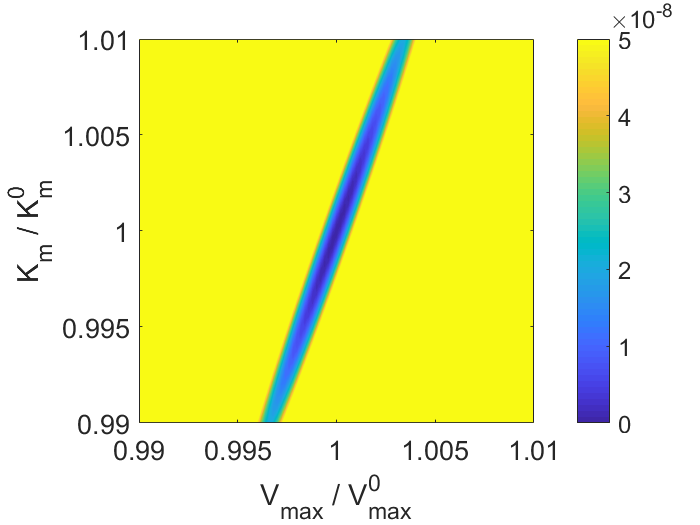
\includegraphics[width=\textwidth]{figure/paper 1/compare6.png}
		\caption{Optimal design in Figure \ref{input3}.}
		\label{SSEopt3}
	\end{subfigure}
	\caption{SSE contours for the optimal experimental designs in Figure \ref{input2} and \ref{input3}.}
	\label{figCompare5}
\end{figure}
\section{Discussion}
\label{Discussion}
{\color{red}In Section \ref{Information}, we mentioned that several design optimality criteria have been proposed in literature. We opted for the D-criterion because it does not depend on the chosen units to describe the model, unlike other criteria such as the A-optimality criterion, which minimizes the average variance of the parameter estimates.} Another criterion that is independent from the chosen units is the I-optimality criterion, which seeks to minimize the average prediction variance over the family of all admissible input profiles {\color{red} \parencite{goos1}}. However, this criterion is computationally more expensive than the D-criterion, which, combined with the already computationally intensive dynamic experimental design idea, would lead to prohibitively long computation times.
\\
\\
In this chapter, we calculated locally optimal designs for a given set of initial values $\mathbf{p}^0$.  Most of the literature on design of experiments for non-linear models focuses on locally optimal design \parencite{fedorov}. This is especially so in the dynamic case \parencite{bernaerts1,bernaerts2,balsa1,balsa2,nahor1,nahor2}. However, we often possess more a priori information concerning a parameter than just a point estimate. For instance, we might also have access to a confidence interval for each model parameter. We could also incorporate this information into our design, with a technique called Bayesian optimal design \parencite{chaloner}, at the expense of a substantial amount of computing time. 
\\
\\
In this chapter, we considered input profiles that are practically feasible. More specifically, when determining the first optimal experimental design, we parametrized our input profile, as a function that could only be on or off. These kinds of input profiles can be easily implemented in practice. We improved on this first design in two different ways: by allowing more than two input levels, and by allowing the input to be switched more rapidly. Similar gains in information were achieved by both improvements, so that there is flexibility in how to perform an informative experiment.
\\
\\
In most of the existing literature, as well as in this chapter, only a single input profile has been optimized \parencite{bernaerts1,bernaerts2,balsa1,balsa2,nahor1,nahor2}. A useful extension of this work would be to optimize multiple input profiles at the same time. Another interesting avenue for future research would be to optimize input profiles for estimating distributed parameter models, which describe the dynamical system by partial differential equations, instead of our lumped approach, which uses ordinary differential equations. {\color{red}The assumption of perfect mixing can then also be relaxed.} Examples of such models are the reaction-diffusion models developed by \textcite{tri2}. To optimize input profiles for such models, however, we first need to develop measures for quantifying parameter uncertainty in these models and for quantifying the information content of the experiments used for collecting the data required for model estimation. (As is often the case in statistics and data science, model development is ahead of tools to verify model quality \parencite{efronhastie}.)
\section{Conclusion}
This chapter presented a pioneering study about the usefulness of optimal dynamic experiments for non-linear modeling in postharvest research. Three D-optimal dynamic experimental designs for the estimation of the Michaelis-Menten respiration parameters of Conference pear were constructed. Each design was constructed using a different parametrization of the input profiles.
\\
\\
The design of protocols for controlled or modified atmosphere of fruit and vegetables is increasingly based on dynamical models of their respiration. Successful implementation depends on accurate knowledge of the model parameters, since every fruit cultivar has to be stored under slightly different conditions. Determining all these conditions is a labor-intensive activity, and requires efficient experimentation. Our three optimal designs show that optimal dynamic design of experiments increases the quality of the respiration parameters' estimates compared to some benchmarks. Therefore, optimal dynamic design of experiments has the potential to facilitate the successful implementation of controlled and modified atmosphere storage. As a matter of fact, dynamic experimentation is a generic method: while our experiments were optimized for Conference pear, a different choice of prior information can be used to obtain optimal input profiles for different cultivars. However, in this chapter, we only took respiration of pear fruit into account. {\color{red}We also used a locally optimal experimental design method which may not be robust. In the next chapter, we improve both these aspects.}